\documentclass{article}
\usepackage{amsfonts, amsmath, amssymb, amsthm, dsfont} % Math notations imported
\usepackage{enumitem}
\usepackage{graphicx}
\usepackage{setspace}
\usepackage{indentfirst}
\usepackage[margin=1in]{geometry}
\graphicspath{{./images/}} % Path to images

% \begin{figure}[htb!]
%      \centering
%      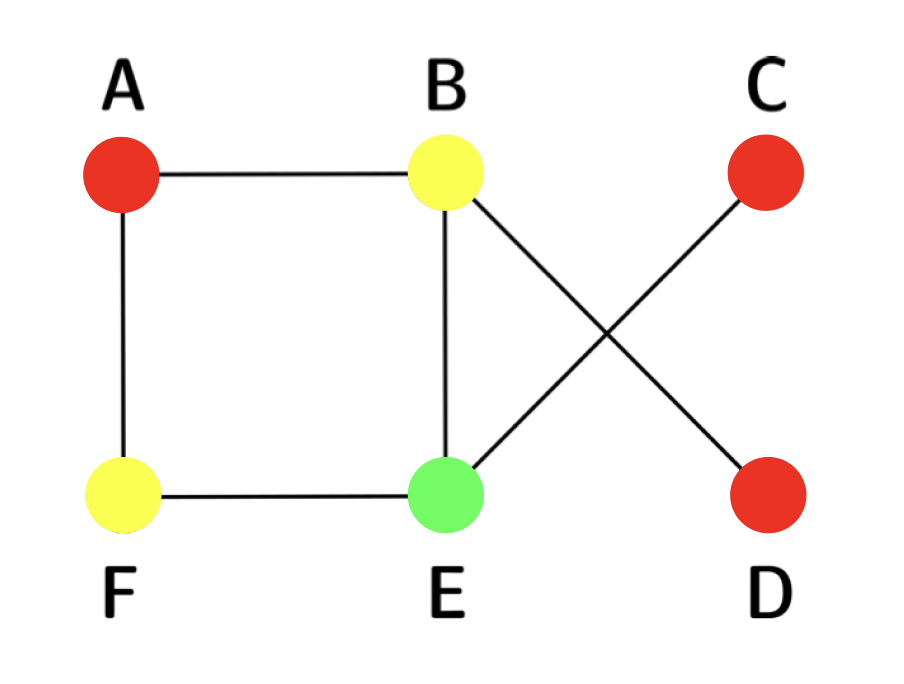
\includegraphics[scale=0.5]{coloring.png}
%      \caption{Coloring of the graph.}
% \end{figure}

% \begin{figure}[htb]
%     \qquad
%     \begin{minipage}{.4\textwidth}
%         \centering
%         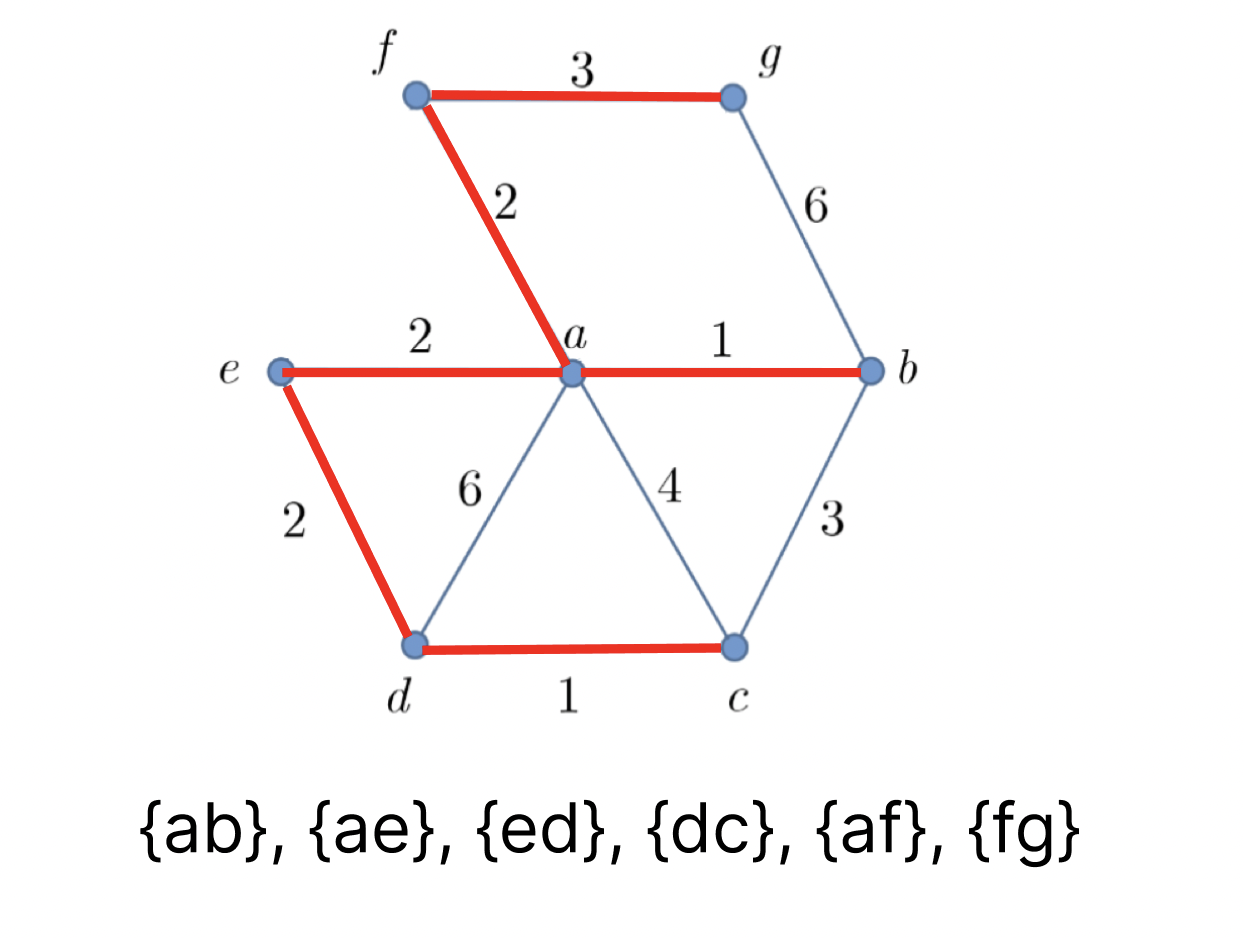
\includegraphics[scale=0.35]{prims.png}
%         \caption{}
%     \end{minipage}    
%     \qquad
%     \begin{minipage}{.4\textwidth}
%         \centering
%         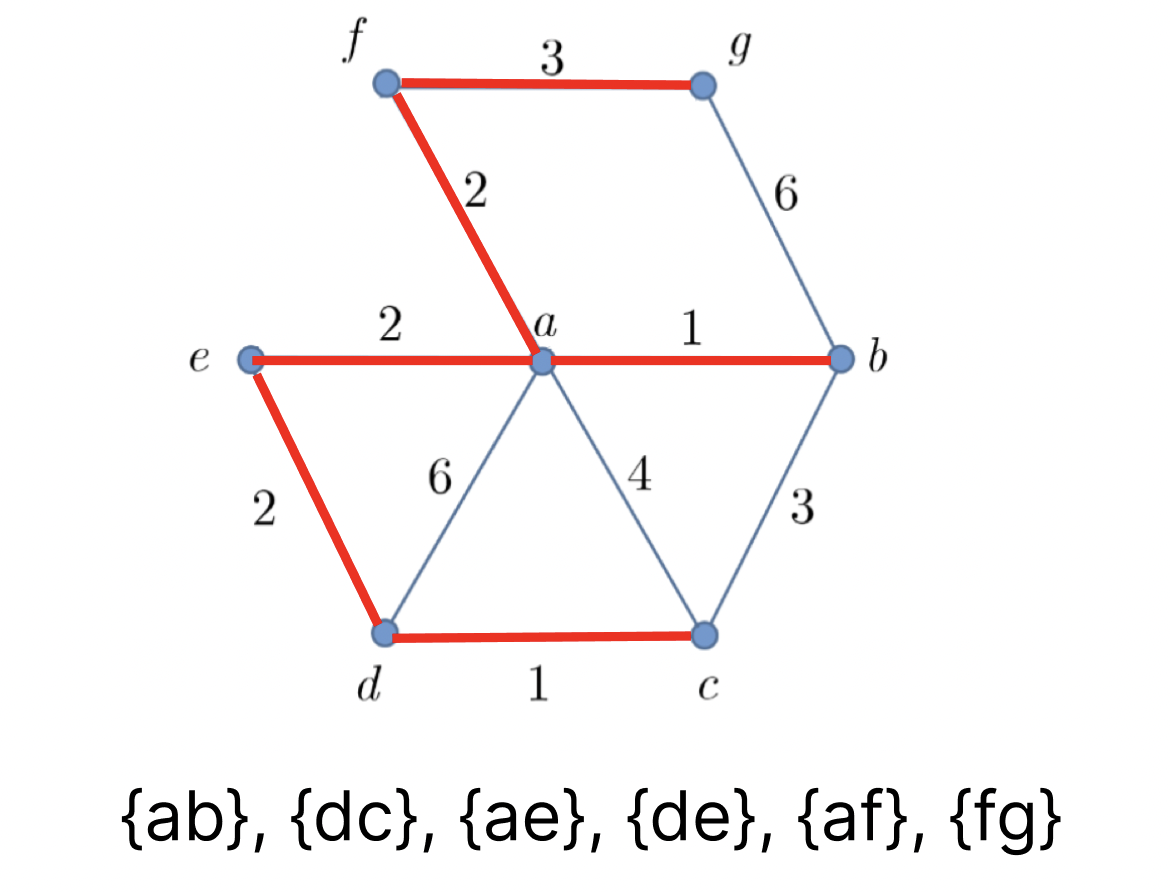
\includegraphics[scale=0.35]{kruskal.png}
%         \caption{}
%     \end{minipage}        
% \end{figure} 

\newtheorem{thm}{Theorem}
\newtheorem{proposition}[thm]{Proposition}
\newtheorem{corollary}[thm]{Corollary}
\newtheorem{lemma}[thm]{Lemma}

\newcommand*{\Var}{\ensuremath{\mathrm{Var}}}
\newcommand*{\Cov}{\ensuremath{\mathrm{Cov}}}
\newcommand*{\Corr}{\ensuremath{\mathrm{Corr}}}
\newcommand*{\Bias}{\ensuremath{\mathrm{Bias}}}
\newcommand*{\MSE}{\ensuremath{\mathrm{MSE}}}
\newcommand*{\range}{\ensuremath{\mathrm{range}}\,}
\newcommand*{\spann}{\ensuremath{\mathrm{span}}\,}
\newcommand*{\nul}{\ensuremath{\mathrm{null}}\,}
\newcommand*{\dom}{\ensuremath{\mathrm{dom}}\,}
\renewcommand*{\implies}{\ensuremath{\Longrightarrow}}
\renewcommand*{\impliedby}{\ensuremath{\Longleftarrow}}
\newcommand*{\Z}{\ensuremath{\mathbb{Z}}}
\newcommand*{\Q}{\ensuremath{\mathbb{Q}}}
\newcommand*{\R}{\ensuremath{\mathbb{R}}}
\newcommand*{\F}{\ensuremath{\mathbb{F}}}
\newcommand*{\C}{\ensuremath{\mathbb{C}}}
\newcommand*{\N}{\ensuremath{\mathbb{N}}}
\newcommand*{\E}{\ensuremath{\mathds{E}}}
\renewcommand*{\P}{\ensuremath{\mathds{P}}}
\newcommand*{\p}{\ensuremath{\mathcal{P}}}

% title information
\title{STAT153 HW4 Sketch}
\author{Neo Lee}
\date{}

\setstretch{1.15}
% main content
\begin{document} 

% placing title information; comment out if using fancyhdr
\maketitle 

$B^kB^\ell x_t = B^kx_{t-\ell} = x_{t-\ell-k} = B^\ell x_{t-k}=B^\ell B^kx_t$

\begin{align*}
    (1 + \phi_1 B + \cdots + \phi_k B^k) (1 + \varphi_1 B + \cdots + \varphi_\ell B^\ell) & = 
    \left(\sum_{i=0}^{k}\phi_i B^i\right) \left(\sum_{j=0}^{\ell}\varphi_j B^j\right) \qquad (\text{let }\phi_0=\varphi_0=1)\\
    & = \sum_{i=0}^{k}\sum_{j=0}^{\ell}\phi_i B^i \cdot \varphi_j B^j \\
    & = \sum_{i=0}^{k}\sum_{j=0}^{\ell}\phi_i\varphi_j \cdot B^i  B^j \\
    & = \sum_{i=0}^{k}\sum_{j=0}^{\ell}\varphi_j\phi_i \cdot B^j  B^i \\
    & = \sum_{i=0}^{k}\sum_{j=0}^{\ell}\varphi_j B^j \cdot \phi_i B^i \\
    & = \sum_{i=0}^{\ell}\sum_{j=0}^{k}\varphi_j B^j \cdot \phi_i B^i \\
    & = (1 + \varphi_1 B + \cdots + \varphi_\ell B^\ell)(1 + \phi_1 B + \cdots + \phi_k B^k) 
\end{align*}

Notice $$\nabla^d\nabla_s^D = (1-B)^d(1-B^s)^D = (1-B^s)^D(1-B)^d$$ where we apply Q2 iteratively on 
$(1+\phi_1 B)$ where $\phi_1 = -1$ and $(1+\varphi_1B + \cdots + \phi_s B^s)$ where $\varphi_s = -1$
and 0 else. 
Therefore, $$\nabla^d\nabla_s^D = \nabla_s^D\nabla^d.$$ Similarly, 
\begin{align*}
    \phi(B)\Phi(B^s)& =(1+\phi_1B + \cdots + \phi_pB^p)(1+\Phi_sB^s +\cdots+ \Phi_{Ps}B^{Ps})\\
    & =(1+\Phi_sB^s +\cdots+ \Phi_{Ps}B^{Ps})(1+\phi_1B + \cdots + \phi_pB^p)
\end{align*}
by apply Q2 iteratively where $\varphi_i = \Phi_i$ for $i=s, 2s, \dots, Ps$ and 0 else. Therefore,
$$\phi(B)\Phi(B^s) = \Phi(B^s)\phi(B).$$
Similarly,
\begin{align*}
    \theta(B)\Theta(B^s)& =(1-\theta_1B - \cdots - \theta_qB^q)(1-\Theta_sB^s -\cdots- \Theta_{Qs}B^{Qs})\\
    & =(1-\Theta_sB^s -\cdots- \Theta_{Qs}B^{Qs})(1-\theta_1B - \cdots - \theta_qB^q),
\end{align*}
by applying Q2 iteratively where $\phi_i = -\theta_i$ and $\varphi_i=-\Theta_i$ for $i=s,\dots,Qs$
and 0 else. Therefore,
$$\theta(B)\Theta(B^s) = \Theta(B^s)\theta(B).$$

Therefore, we achieved the desired equivalence.


$$\forall t, \nabla x_t = u \implies x_t = x_{t-1} + u = x_{t-2} + u + u = x_{t-3} + u + u + u = \cdots = x_0 + tu,$$
which is in the desired form of $x_t = a+bt$.

\begin{align*}
    x_t & = u + vt + x_{t-1} \\
    & = u + vt + u + v(t-1) + x_{t-2} \\
    & = u + vt + u + v(t-1) + u + v(t-2) + x_{t-3} \\
    & = u + vt + u + v(t-1) + u + v(t-2) + \cdots + u + v(t-(t-1)) + x_0 \\
    & = ut + v\left(t^2 - (1 + \cdots + (t-1))\right) + x_0 \\
    & = ut + v\left(t^2 - \frac{t(t-1)}{2}\right) + x_0 \\
    & = ut + v\left(\frac{t^2 + t}{2}\right) + x_0 \\
    & = x_0 + \left(u + \frac{v}{2}\right)t + \frac{v}{2}t^2,
\end{align*}
which is in the desired form of $x_t = a + bt + ct^2$.

$$(1-\phi B)x_t = (1 + \theta B)w_t \implies 
x_t - \phi x_{t-1} = w_t + \theta w_{t-1} \implies
x_t = \phi x_{t-1} + w_t + \theta w_{t-1}.$$

Then, 
\begin{align*}
    \hat{x}_{t+1|t} & = \hat{\phi}x_t + w_{t+1} + \hat{\theta}w_t = 
    \hat{\phi}x_t + \hat{\theta}w_t \qquad (w_{t+1} = 0) \\
    \hat{x}_{t+2|t} & = \hat{\phi}x_{t+1|t} + w_{t+2} + \hat{\theta}w_{t+1} =
    \hat{\phi}\left(\hat{\phi}x_t + \hat{\theta}w_t\right) \qquad (w_{t+2} =w_{t+1} = 0) \\
    \hat{x}_{t+3|t} & = \hat{\phi}x_{t+2|t} + w_{t+3} + \hat{\theta}w_{t+2} =
    \hat{\phi}\left(\hat{\phi}\left(\hat{\phi}x_t + \hat{\theta}w_t\right)\right) \qquad (w_{t+3} =w_{t+2} = 0) \\
    &\quad \vdots \\
    \lim_{h\to\infty}\hat{x}_{t+h|t} & = \lim_{h\to\infty}\hat{\phi}^{h}x_t +
    \hat{\phi}^{h-1}\hat{\theta}w_t = 0 \qquad (\because \hat{\phi} < 1 \text{ and } x_t, \hat{\theta}w_t\in\mathbb{R})
\end{align*}

$$(1-\phi B)x_t=c+(1+\theta B)w_t \implies x_t = \phi x_{t-1} + w_t + \theta w_{t-1} + c.$$

Then, 
\begin{align*}
    \hat{x}_{t+1|t} & = \hat{\phi}x_t + w_{t+1} + \hat{\theta}\hat{w_t} + c = 
    \hat{\phi}x_t + \hat{\theta}\hat{w_t} + c \qquad (w_{t+1} = 0) \\
    \hat{x}_{t+2|t} & = \hat{\phi}x_{t+1|t} + w_{t+2} + \hat{\theta}w_{t+1} + c =
    \hat{\phi}\left(\hat{\phi}x_t + \hat{\theta}\hat{w_t}+c\right)+c \qquad (w_{t+2} =w_{t+1} = 0) \\
    \hat{x}_{t+3|t} & = \hat{\phi}x_{t+2|t} + w_{t+3} + \hat{\theta}w_{t+2}+c =
    \hat{\phi}\left(\hat{\phi}\left(\hat{\phi}x_t + \hat{\theta}\hat{w_t}+c\right)+c\right)+c \qquad (w_{t+3} =w_{t+2} = 0) \\
    &\quad \vdots \\
    \hat{x}_{t+h|t} & = \hat{\phi}^hx_t + \hat{\phi}^{h-1}\hat{\theta}\hat{w_t}+ c\cdot\sum_{k=0}^{h-1}\hat{\phi}^k \\
    \lim_{h\to\infty}\hat{x}_{t+h|t} & = \lim_{h\to\infty}\hat{\phi}^hx_t + \hat{\phi}^{h-1}\hat{\theta}\hat{w_t}+ c\cdot\sum_{k=0}^{h-1}\hat{\phi}^k =
    c\cdot\lim_{h\to\infty}\sum_{k=0}^{h-1}\hat{\phi}^k = C,
\end{align*}
because $\hat{\phi} < 1$, $\hat{\theta}w_t\in\mathbb{R}$, and 
$\lim_{h\to\infty}\sum_{k=0}^{h-1}\hat{\phi}^k$ converges to some real number.

$$\emph{rows} = t_0 + (t_0 + 1) + (t_0 + 2) + \cdots + n = \frac{(t_0 + n)(n-t_0+1)}{2}.$$

$\underline{c=0, d=1}:$
Let $y_t = \nabla x_t$, then 
$$(1-\phi B)\nabla x_t = (1+\theta B)w_t \Leftrightarrow (1-\phi B)y_t = (1+\theta B)w_t.$$
By Q9, $\hat{y}_{t+h|t}= 0$ as $h\to\infty$, thus $\nabla \hat{x}_{t+h|t}=0$ as $h\to\infty$.
By Q5, $\hat{x}_{t+h|t}$ approaches a constant sequence as $h\to\infty$.

$\underline{c=0, d=2}:$
Let $y_t = \nabla^2 x_t$, then 
$$(1-\phi B)\nabla^2 x_t = (1+\theta B)w_t \Leftrightarrow (1-\phi B)y_t = (1+\theta B)w_t.$$
By Q9, $\hat{y}_{t+h|t}= 0$ as $h\to\infty$, thus $\nabla^2 \hat{x}_{t+h|t}=0$ as $h\to\infty$.
Notice $\nabla^2\hat{x}_{t+h|t} = \nabla(\nabla\hat{x}_{t+h|t})$, then by Q5, 
$\nabla\hat{x}_{t+h|t}$ approaches a constant sequence as $h\to\infty$. Further, by Q6,
$\hat{x}_{t+h|t}$ approaches a linear function of $t$ as $h\to\infty$.

$\underline{c\neq0, d=1}:$
Let $y_t = \nabla x_t$, then 
$$(1-\phi B)\nabla x_t = c + (1+\theta B)w_t \Leftrightarrow (1-\phi B)y_t = c + (1+\theta B)w_t.$$
By Q10, $\hat{y}_{t+h|t}$ approaches a non-zero constant as $h\to\infty$, thus $\nabla \hat{x}_{t+h|t}$ 
approaches a none-zero constant as $h\to\infty$.
By Q6, $\hat{x}_{t+h|t}$ approaches a linear function of $t$ as $h\to\infty$.

$\underline{c\neq0, d=2}:$
Let $y_t = \nabla^2 x_t$, then 
$$(1-\phi B)\nabla x_t = c + (1+\theta B)w_t \Leftrightarrow (1-\phi B)y_t = c + (1+\theta B)w_t.$$
By Q10, $\hat{y}_{t+h|t}$ approaches a non-zero constant as $h\to\infty$, thus $\nabla^2 \hat{x}_{t+h|t}$ 
approaches a none-zero constant as $h\to\infty$.
By Q8, $\hat{x}_{t+h|t}$ approaches a quadratic function of $t$ as $h\to\infty$.
\end{document}
